\documentclass[border=12pt]{standalone}
\def\pgfsysdriver{pgfsys-dvisvgm.def}
\usepackage[dvisvgm]{xcolor}
\usepackage{xeCJK}
\setCJKmainfont{HaranoAjiGothic-Regular.otf}[BoldFont=HaranoAjiGothic-Bold.otf]
\setCJKsansfont{HaranoAjiGothic-Regular.otf}[BoldFont=HaranoAjiGothic-Bold.otf]
\usepackage{amsmath,amssymb,tikz,lmodern}
\usetikzlibrary{arrows.meta,positioning,calc,fit,backgrounds}
\renewcommand{\familydefault}{\sfdefault}
\definecolor{ink}{HTML}{25322F}
\definecolor{green}{HTML}{246657}
\definecolor{tint}{HTML}{EEF4F0}
\definecolor{soft}{HTML}{C6D2CC}
\definecolor{muted}{HTML}{52615B}
\newif\ifJapanese
\newcommand{\Tx}[2]{\ifJapanese #1\else #2\fi}
\newcommand{\Eff}{\overline{\operatorname{Eff}}}
\newcommand{\heading}[3]{{\color{green}\bfseries #1\quad\Tx{#2}{#3}}\\[5pt]}
% A white rectangle makes the complete citation label clickable, including spaces.
\newcommand{\refurl}[2]{\special{dvisvgm:raw <a xlink:href="#1" target="_blank" rel="noopener noreferrer">}{\setlength{\fboxsep}{0pt}\colorbox{white}{\color{green}\underline{\strut #2}}}\special{dvisvgm:raw </a>}}
\tikzset{
 card/.style={draw=soft,fill=white,rounded corners=2pt,align=left,text=ink,font=\fontsize{10.5}{14}\selectfont,inner xsep=12pt,inner ysep=10pt,text width=14.4cm},
 half/.style={card,text width=6.45cm,minimum height=2.05cm},
 result/.style={card,draw=green,fill=tint,line width=.9pt},
 reason/.style={align=left,text=muted,font=\fontsize{9}{12}\selectfont,inner sep=0pt,text width=12.7cm},
 branchreason/.style={reason,text width=5.95cm},
 edge/.style={-{Stealth[length=2.4mm]},draw=green,line width=1pt},
 wire/.style={draw=green,line width=1pt},
}
% Keep the arrow in a dedicated left gutter; explanations never cover it.
\newcommand{\flow}[3]{
 \coordinate (#2-from) at ($(#1.south)+(-6.9,0)$);
 \coordinate (#2-to) at ($(#2.north)+(-6.9,0)$);
 \draw[edge] (#2-from)--(#2-to);
 \node[reason,anchor=west] (#2-reason) at ($(#2-from)!.5!(#2-to)+(.55,0)$) {#3};
}

\newcommand{\Cite}[2]{\refurl{#1}{#2}}

\Japanesetrue
\begin{document}
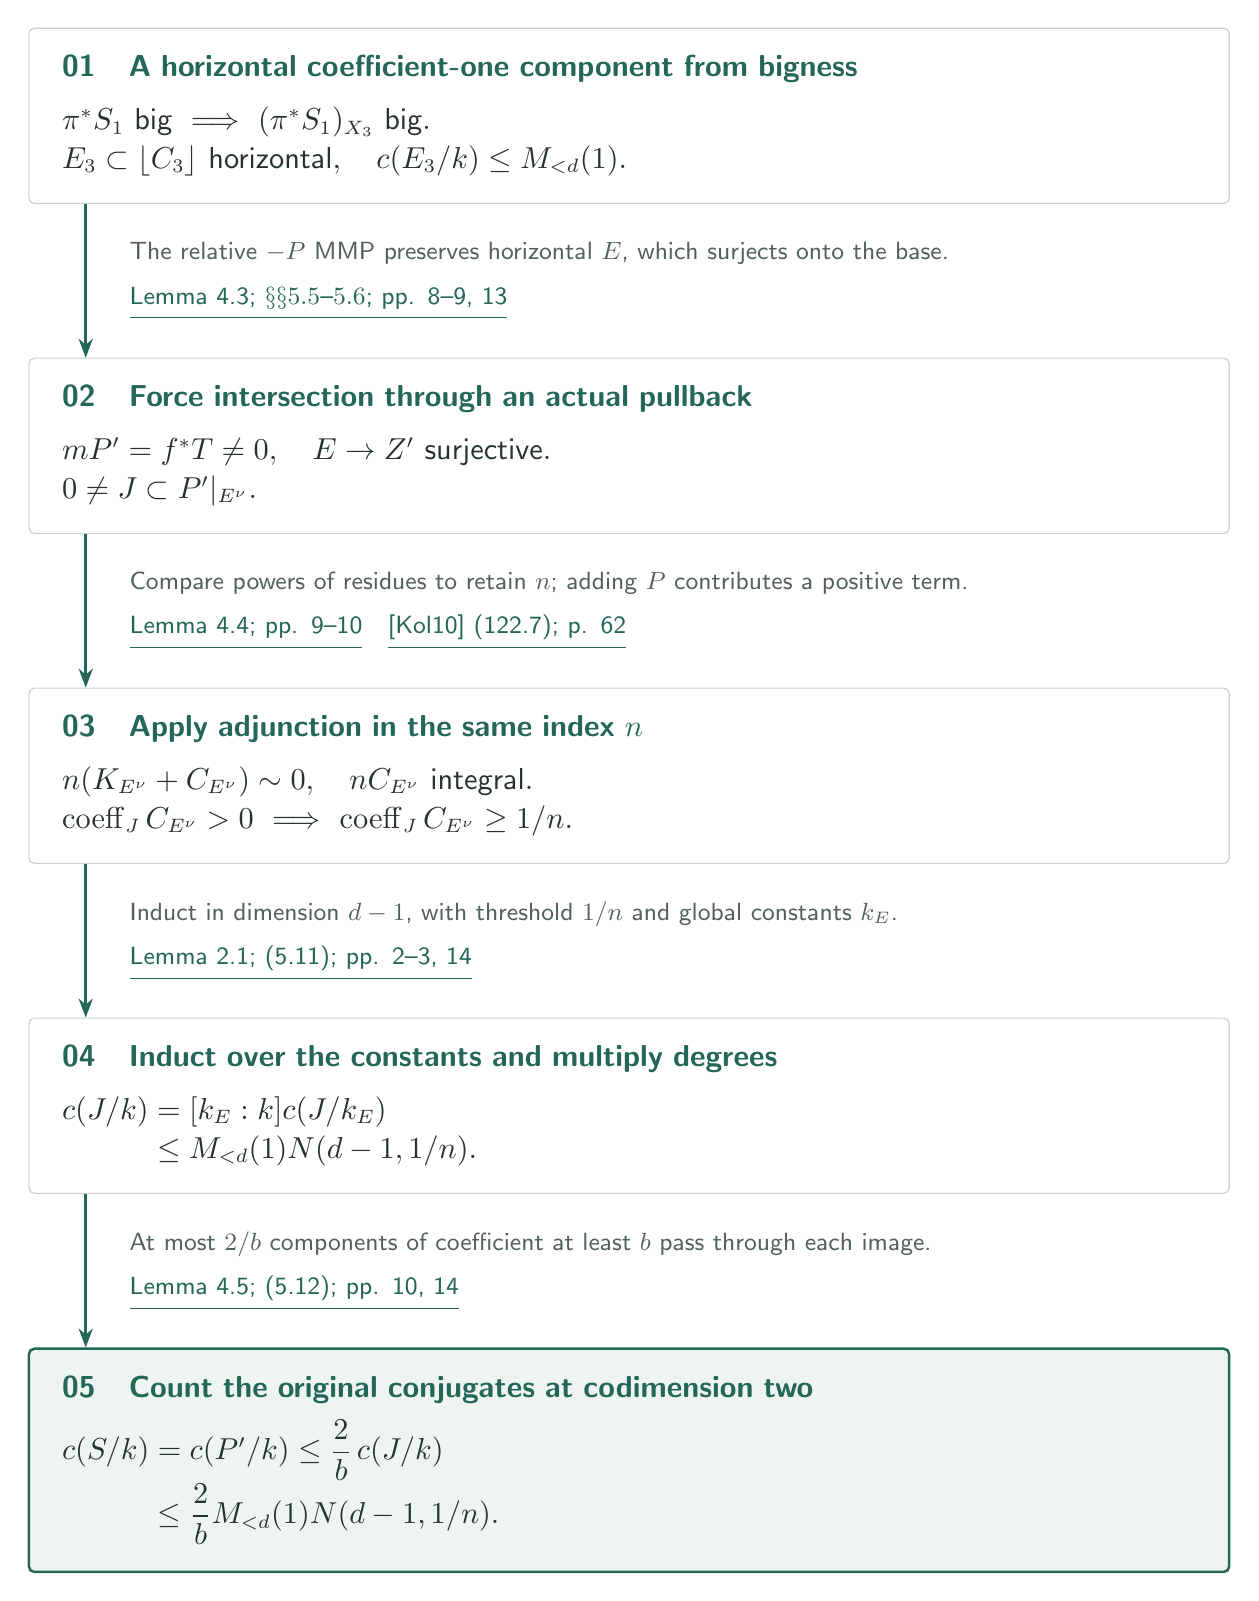
\begin{tikzpicture}
\node[card] (n0) {\heading{01}{bigな因子から水平係数1成分}{A horizontal coefficient-one component from bigness}$\pi^*S_1\text{ big}\ \Longrightarrow\ (\pi^*S_1)_{X_3}\text{ big}.$\\ $E_3\subset\lfloor C_3\rfloor\text{ horizontal},\quad c(E_3/k)\le M_{<d}(1).$};
\node[card,below=1.95cm of n0] (n1) {\heading{02}{交差を実際の引戻しで作る}{Force intersection through an actual pullback}$mP'=f^*T\ne0,\quad E\to Z'\text{ surjective}.$\\ $0\ne J\subset P'|_{E^\nu}.$};
\flow{n0}{n1}{\Tx{垂直な $-P$ のMMPは水平な $E$ を保存し、$E$ は底に全射。}{The relative $-P$ MMP preserves horizontal $E$, which surjects onto the base.}\\[4pt]\Cite{https://github.com/openai/math/blob/adc7f1241b42e322a6451854ab7e4b4c146bf78a/preprints/Arithmetic-Stein-degree-bounds-for-log-Calabi-Yau-pairs-September-25-2026/paper.pdf}{Lemma 4.3; $\S\S5.5$--$5.6$; pp. 8--9, 13}}
\node[card,below=1.95cm of n1] (n2) {\heading{03}{同じ指数 $n$ で随伴}{Apply adjunction in the same index $n$}$n(K_{E^\nu}+C_{E^\nu})\sim0,\quad nC_{E^\nu}\text{ integral}.$\\ $\operatorname{coeff}_{J}C_{E^\nu}>0\ \Longrightarrow\ \operatorname{coeff}_{J}C_{E^\nu}\ge1/n.$};
\flow{n1}{n2}{\Tx{留数の冪の比較で指数を保存。$P$ を加えるとdifferentに正の項が入る。}{Compare powers of residues to retain $n$; adding $P$ contributes a positive term.}\\[4pt]\Cite{https://github.com/openai/math/blob/adc7f1241b42e322a6451854ab7e4b4c146bf78a/preprints/Arithmetic-Stein-degree-bounds-for-log-Calabi-Yau-pairs-September-25-2026/paper.pdf}{Lemma 4.4; pp. 9--10}\quad \Cite{https://web.math.princeton.edu/~kollar/book/chap2.pdf#page=62}{[Kol10] (122.7); p. 62}}
\node[card,below=1.95cm of n2] (n3) {\heading{04}{定数体上の帰納と次数の積}{Induct over the constants and multiply degrees}$c(J/k)=[k_E:k]c(J/k_E)$\\ $\hphantom{c(J/k)}\le M_{<d}(1)N(d-1,1/n).$};
\flow{n2}{n3}{\Tx{次元 $d-1$、係数下限 $1/n$、大域関数体 $k_E$ で帰納。}{Induct in dimension $d-1$, with threshold $1/n$ and global constants $k_E$.}\\[4pt]\Cite{https://github.com/openai/math/blob/adc7f1241b42e322a6451854ab7e4b4c146bf78a/preprints/Arithmetic-Stein-degree-bounds-for-log-Calabi-Yau-pairs-September-25-2026/paper.pdf}{Lemma 2.1; (5.11); pp. 2--3, 14}}
\node[result,below=1.95cm of n3] (n4) {\heading{05}{余次元2で元の共役数を数える}{Count the original conjugates at codimension two}$c(S/k)=c(P'/k)\le\dfrac2b\,c(J/k)$\\ $\hphantom{c(S/k)}\le\dfrac2b M_{<d}(1)N(d-1,1/n).$};
\flow{n3}{n4}{\Tx{各共役の像を通る係数 $\ge b$ の成分は高々 $2/b$ 個。}{At most $2/b$ components of coefficient at least $b$ pass through each image.}\\[4pt]\Cite{https://github.com/openai/math/blob/adc7f1241b42e322a6451854ab7e4b4c146bf78a/preprints/Arithmetic-Stein-degree-bounds-for-log-Calabi-Yau-pairs-September-25-2026/paper.pdf}{Lemma 4.5; (5.12); pp. 10, 14}}
\end{tikzpicture}

\end{document}
